\documentclass{article}
\usepackage{listings}
\usepackage{color}
\usepackage{keyval}
\definecolor{dkgreen}{rgb}{0,0.6,0}
\definecolor{gray}{rgb}{0.5,0.5,0.5}
\definecolor{mauve}{rgb}{0.58,0,0.82}
\usepackage{bookmark}
\usepackage{amsmath}
\usepackage{geometry}
\usepackage{hyperref}
\usepackage{listings}
\usepackage{xcolor}
\usepackage{graphicx}
\usepackage{amsfonts}

\lstset{
  basicstyle=\footnotesize, 
  numbers=left, 
  numberstyle=\tiny\color{gray}, 
  stepnumber=1,
  numbersep=5pt, 
  backgroundcolor=\color{white},
  showspaces=false,
  showstringspaces=false,
  showtabs=false,
  frame=shadowbox,
  rulecolor=\color{black},
  tabsize=2,
  captionpos=b,
  breaklines=true, 
  breakatwhitespace=false, 
  title=\lstname,
  keywordstyle=\color{blue},
  commentstyle=\color{dkgreen},
  escapeinside={\%*}{*)}, 
  morekeywords={*,...} 
}

\begin{document}

To compare the performace of different sorting algorithms, I generated arrays in sizes of 1-100, and for each of the sizes ther eare 100 cases. The following figure shows the performace of the algorithms for different scales on the size of arrays.

\begin{figure}[htbp]
    \begin{minipage}[t]{0.3\textwidth}
        \centering
        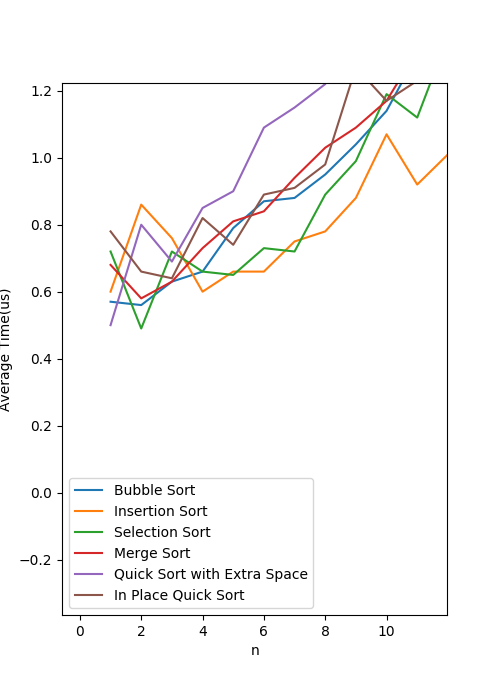
\includegraphics[width=\textwidth]{zero_ten.png}
        \caption{1-10}
    \end{minipage}
    \begin{minipage}[t]{0.35\textwidth}
        \centering
        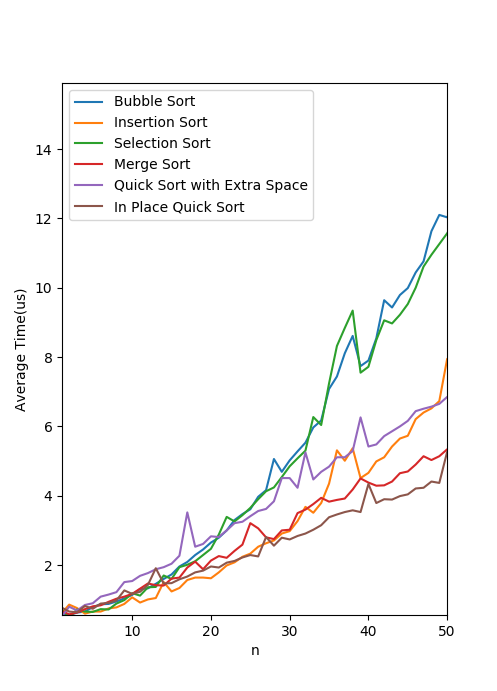
\includegraphics[width=\textwidth]{zero_fifty.png}
        \caption{1-50}
    \end{minipage}
    \begin{minipage}[t]{0.35\textwidth}
        \centering
        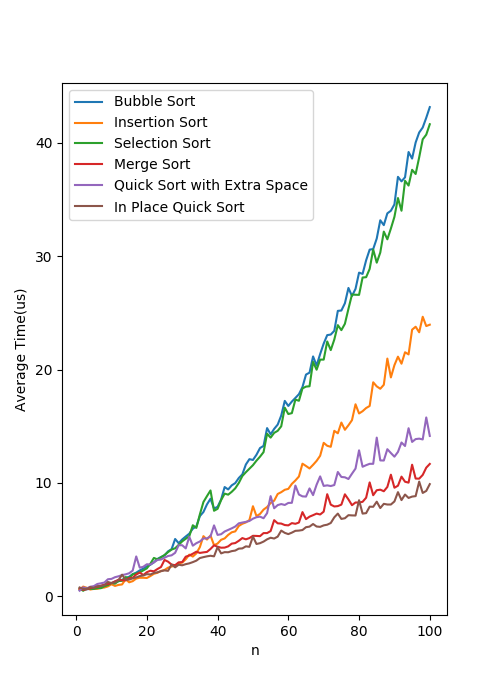
\includegraphics[width=\textwidth]{zero_hundred.png}
        \caption{1-100}
    \end{minipage}
\end{figure}

When the size of the array is small, it seems that insertion sort and selection sort have a relatively higher performance. And those $O(nlogn)$ algorithms are actually slower. It is mainly because that those algorithms all need recursive call and some has extra space to allocate, and the process of memory allocation to the recursice function or data will be time-consuming. 

When the size grows larger, it can be seen that selection sort, bubble sort and insertion sort's time grows a lot faster than the other three. So the $O(nlogn)$ complexity begins to take advantage when the size is big.

Among the three $O(n^2)$ algorithms, it can be seen that insertion sort is much faster than the other two. I believe it is because of the implementation. When I implement the insertion sort, the finding and shifting operations are combined, so that the time of this algorithm can be reduced.

The in-place quick sort works the fastest when the size is large. It also makes sense because it avoid the time and space consumption of extra space.

So in conclusion, When the size is small, the insertion sort and selection sort works well enough. And when the size becomes larger, those $O(nlogn)$ complexity algorithms will have more advantage. And functions with less extra space allocation will be faster than those with more.

The source code are attached in the pages following.

\newpage

{\bf 1. Source Code for algorithms and main function.}
\begin{lstlisting}[title=main.cpp,language=C++]
#include "sorting.h"
#include "clocking.h"
//#define CLOCKED
using namespace std;

int main(){
    srand(time(NULL));
#ifdef CLOCKED
    clocking_main();
#else
    void (*func[6]) (int *arr,int n) = {
        bubble_sort,
        insertion_sort,
        selection_sort,
        merge_sort,
        quick_sort,
        quick_sort_inplace
    };
    int mode,n,*arr;
    cin >> mode >> n;
    if (n==0) return 0;
    arr = new int [n];
    for (int i=0;i<n;i++) cin >> arr[i];
    func[mode](arr,n);
    for (int i=0;i<n;i++) cout << arr[i] << endl;
#endif
    return 0;
}    
\end{lstlisting}
\begin{lstlisting}[title=sorting.h,language=C++]
#ifndef SORTING_H
#define SORTING_H
#include<iostream>
#include<cstdlib>
#include<fstream>
#include<sstream>
#include<ctime>
#define SWAP(a,b) {if (a!=b){a = a^b;b =  a^b;a = a^b;} }
void bubble_sort(int *arr,int n);
void insertion_sort(int *arr,int n);
void selection_sort(int *arr,int n);
void merge_sort(int *arr,int n);
void quick_sort(int *arr,int n);
void quick_sort_inplace(int *arr,int n);
#endif
\end{lstlisting}
\begin{lstlisting}[title=sorting.cpp,language=C++]
#include "sorting.h"
using namespace std;

void bubble_sort(int *arr,int n){
    for (int i=n;i>0;i--)
        for (int j=0;j<i-1;j++)
            if (arr[j]>arr[j+1]) SWAP(arr[j],arr[j+1]);
}

void insertion_sort(int *arr,int n){
    for (int i=1;i<n;i++)
        for (int j=i;(j>0)&&(arr[j]<arr[j-1]);j--) SWAP(arr[j],arr[j-1]);
}

void selection_sort(int *arr, int n){
    for (int i=0;i<n-1;i++)
        for (int j=i+1;j<n;j++)
            if (arr[i]>arr[j]) SWAP(arr[j],arr[i]);
}

void merge_sort(int *arr,int n){
    if (n==1) return;
    int left = n/2;
    int right = n-left;
    merge_sort(arr,left);
    merge_sort(arr+left,right);
    int *tmp = new int[n];
    int lflag=0,rflag=left,flag=0;
    while ((lflag!=left)||(rflag!=n)){
        if (lflag==left){
            tmp[flag] = arr[rflag];
            flag++;rflag++;
        }
        else if (rflag==n){
            tmp[flag] = arr[lflag];
            flag++;lflag++;
        }
        else if (arr[rflag]<arr[lflag]){
            tmp[flag] = arr[rflag];
            flag++;rflag++;
        }
        else {
            tmp[flag] = arr[lflag];
            flag++;lflag++;
        }
    }
    for (int i=0;i<n;i++) arr[i] = tmp[i];
    delete [] tmp;
}

void quick_sort(int *arr,int n){
    if ((n==0)||(n==1)) return;
    if (n==2){
        if (arr[0]>arr[1]) SWAP(arr[0],arr[1]);
        return;
    }
    int pivot = rand()%n;
    int *arrl = new int[n];
    int *arrr = new int[n];
    int lflag=0,rflag=0;
    for (int i=0;i<n;i++){
        if (arr[i]<arr[pivot]) {
            arrl[lflag] = arr[i];
            lflag++;
        }
        else if ((arr[i]>=arr[pivot])&&(i!=pivot)) {
            arrr[rflag] = arr[i];
            rflag++;
        }
    }
    quick_sort(arrl,lflag);
    quick_sort(arrr,rflag);
    int tmp = arr[pivot];
    for (int i=0;i<lflag;i++) arr[i] = arrl[i];
    arr[lflag] = tmp;
    for (int i=lflag+1;i<n;i++) arr[i] = arrr[i-lflag-1];
    delete [] arrl;
    delete [] arrr;
}

void quick_sort_inplace(int *arr, int n){
    if ((n==0)||(n==1)) return;
    if (n==2){
        if (arr[0]>arr[1]) SWAP(arr[0],arr[1]);
        return;
    }
    int pivot = rand()%n;
    SWAP(arr[pivot],arr[0]);
    int lflag=1,rflag=n-1;
    while (lflag<rflag){
        while ((arr[lflag]<arr[0])&&(lflag<n-1)) lflag++;
        while ((arr[rflag]>=arr[0])&&(rflag>0)) rflag--;
        if (lflag<rflag) SWAP(arr[lflag],arr[rflag]);
    }
    SWAP(arr[0],arr[rflag]);
    quick_sort_inplace(arr,rflag);
    quick_sort_inplace(arr+rflag+1,n-rflag-1);
}
\end{lstlisting}
\begin{lstlisting}[title=clocking.h,language=C++]
#ifndef CLOCKING_H
#define CLOCKING_H
#include "sorting.h"
void clocking_main();
#endif
\end{lstlisting}
\begin{lstlisting}[title=clocking.h,language=C++]
#include "sorting.h"
#include <string>
using namespace std;

string int_to_string(int x){
	ostringstream sout;
	sout<<x;
	return sout.str();
}

void clocking_main(){
	void (*func[6]) (int *arr,int n) = {
		bubble_sort,
		insertion_sort,
		selection_sort,
		merge_sort,
		quick_sort,
		quick_sort_inplace
	};
	double table[6][100];
	for (int i=0;i<6;i++)
		for (int j=0;j<100;j++)
			table[i][j] = 0;
	string number[101];
	for (int i=0;i<101;i++) number[i]= int_to_string(i);
	for (int i=0;i<6;i++) {
		cout << "Checking Mode " << i << endl;
		for (int j=1;j<=100;j++){
			cout << "Checking number " << j << endl;
			for (int k=0;k<100;k++){
				string name = "p1/"+number[j]+"/"+number[i]+"/"+number[k]+"/test.in";
				ifstream fin;
				fin.open(name.c_str());
				int *arr,n,mode;
				fin >> mode >> n;
				arr = new int[n];
				for (int x = 0;x<n;x++) fin >> arr[x];
				int now = clock();
				func[mode](arr,n);
				int duration = clock()-now;
				table[mode][j-1]+=(double)duration/(double)CLOCKS_PER_SEC*1000.0;
				fin.close();
				delete []arr;
			}
		}
	}
	ofstream fout;
	fout.open("result.out");
	for (int i=0;i<6;i++){
		for (int j=0;j<100;j++) fout << table[i][j]/100.0 << " ";
		fout << endl;
	}
	fout.close();
}
\end{lstlisting}
{\bf 2. Code to generate random cases(Matlab)}
\begin{lstlisting}[title=randcase.m,language=Matlab]
for i = 1:100
mkdir(num2str(i));
for j = 0:5
    mkdir([num2str(i),'\',num2str(j)]);
end
for k = 0:99
    seq = randi([-1000,1000],1,i);
    for j = 0:5
        mkdir([num2str(i),'\',num2str(j),'\',num2str(k)]);
        fout = fopen([num2str(i),'\',num2str(j),'\',num2str(k),'\test.in'],"w+");
        fprintf(fout,"%d\n%d\n",j,i);
        for l=1:i
            fprintf(fout,"%d\n",seq(l));
        end
        fclose(fout);
    end
end
\end{lstlisting}
{\bf 3. Plot the curves of the run time with respect to size(Python)}
\begin{lstlisting}[title=printresult.py,language=Python]
import numpy as np
import matplotlib.pyplot as plt

a = np.loadtxt('result.out')
namelist = ['Bubble Sort','Insertion Sort','Selection Sort','Merge Sort','Quick Sort with Extra Space','In Place Quick Sort']

plt.figure(1)
for i in range(6):
    plt.plot(np.linspace(1,100,100),a[i]*1000,label=namelist[i])
plt.xlabel('n')
plt.ylabel('Average Time(us)')
plt.legend()
plt.show()    
    \end{lstlisting}
\end{document}